% Created 2018-12-17 lun 13:15
% Intended LaTeX compiler: pdflatex
\documentclass[xcolor={usenames,svgnames,dvipsnames}]{beamer}
\usepackage[utf8]{inputenc}
\usepackage[T1]{fontenc}
\usepackage{graphicx}
\usepackage{grffile}
\usepackage{longtable}
\usepackage{wrapfig}
\usepackage{rotating}
\usepackage[normalem]{ulem}
\usepackage{amsmath}
\usepackage{textcomp}
\usepackage{amssymb}
\usepackage{capt-of}
\usepackage{hyperref}
\usepackage{color}
\usepackage{listings}
\usepackage{mathpazo}
\usepackage{gensymb}
\usepackage{amsmath}
\usepackage{esdiff}
\usepackage{steinmetz}
\bibliographystyle{plain}
\AtBeginSubsection[]{\begin{frame}[plain]\tableofcontents[currentsubsection,sectionstyle=show/shaded,subsectionstyle=show/shaded/hide]\end{frame}}
\AtBeginSection[]{\begin{frame}[plain]\tableofcontents[currentsection,hideallsubsections]\end{frame}}
\usepackage[emulate=units]{siunitx}
\sisetup{fraction=nice, decimalsymbol=comma, retain-unity-mantissa = false}
\newunit{\wattpeak}{Wp}
\newunit{\watthour}{Wh}
\newunit{\amperehour}{Ah}
\hypersetup{colorlinks=true, linkcolor=Blue, urlcolor=Blue}
\renewcommand{\thefootnote}{\fnsymbol{footnote}}
\beamertemplatenavigationsymbolsempty
\setbeamertemplate{footline}[frame number]
\newcommand{\laplace}[1]{\mathbf{#1}(\mathbf{s})}
\newcommand{\slp}{\mathbf{s}}
\newcommand{\fasor}[1]{\mathbf{#1}(\omega)}
\newcommand{\atan}{\mathrm{atan}}
\setbeamercolor{alerted text}{fg=blue!50!black} \setbeamerfont{alerted text}{series=\bfseries}
\usetheme[hideothersubsections]{Goettingen}
\usecolortheme{rose}
\usefonttheme{serif}
\author{Oscar Perpiñán Lamigueiro}
\date{Noviembre 2018}
\title{Respuesta en Frecuencia}
\subtitle{Teoría de Circuitos III}
\hypersetup{
 pdfauthor={Oscar Perpiñán Lamigueiro},
 pdftitle={Respuesta en Frecuencia},
 pdfkeywords={},
 pdfsubject={},
 pdfcreator={Emacs 25.2.2 (Org mode 9.1.13)}, 
 pdflang={Spanish}}
\begin{document}

\maketitle

\section{Introducción}
\label{sec:org6edc6b6}
\begin{frame}[label={sec:orgd5fe243}]{Introducción}
\begin{block}{Respuesta en Frecuencia}
La respuesta en frecuencia de un circuito es la variación del comportamiento del circuito a los cambios de la frecuencia de alimentación.
\end{block}

\begin{itemize}
\item Hasta ahora hemos analizado circuitos alimentados por generadores con frecuencia constante.
\item El análisis de la \alert{respuesta en frecuencia} consiste en variar la frecuencia de alimentación y estudiar la respuesta.
\item Este análisis se realiza en \alert{régimen permanente} con señales sinusoidales.
\end{itemize}
\end{frame}


\section{Función de Transferencia}
\label{sec:org62e152e}
\begin{frame}[label={sec:org1319266}]{Función de Transferencia}
\[
  \laplace{H}\rvert_{\slp = j\omega} = \frac{\laplace{Y}}{\laplace{X}}
\]

\begin{center}
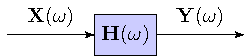
\includegraphics[width=.9\linewidth]{../figs/TransferFunction.pdf}
\end{center}


\begin{columns}
\begin{column}{0.5\columnwidth}
\begin{center}
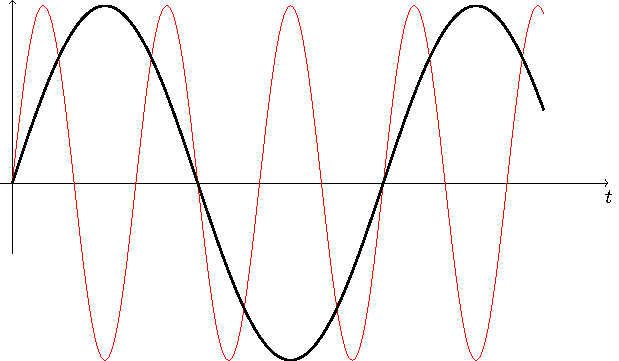
\includegraphics[width=.9\linewidth]{../figs/sinX.pdf}
\end{center}
\end{column}

\begin{column}{0.5\columnwidth}
\begin{center}
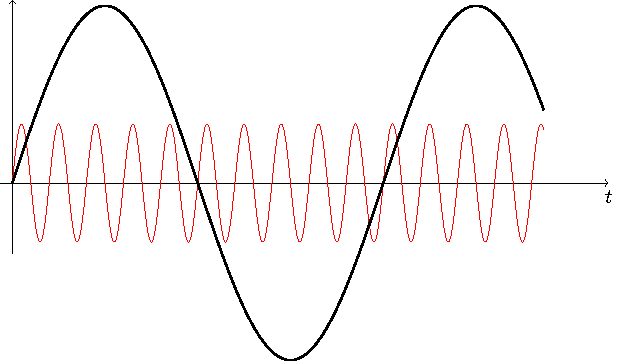
\includegraphics[width=.9\linewidth]{../figs/sinY.pdf}
\end{center}
\end{column}
\end{columns}
\end{frame}

\begin{frame}[label={sec:org2cf626e}]{Funciones de Transferencia}
\begin{itemize}
\item Ganancia de Tensión
\end{itemize}
\[
\laplace{H} =\frac{\laplace{V_o}}{\laplace{V_i}}
\]
\begin{itemize}
\item Ganancia de Corriente
\end{itemize}
\[
\laplace{H} =\frac{\laplace{I_o}}{\laplace{I_i}}
\]
\begin{itemize}
\item Impedancia de Transferencia
\end{itemize}
\[
\laplace{H} =\frac{\laplace{V_o}}{\laplace{I_i}}
\]
\begin{itemize}
\item Admitancia de Transferencia
\end{itemize}
\[
\laplace{H} =\frac{\laplace{I_o}}{\laplace{V_i}}
\]
\end{frame}

\begin{frame}[label={sec:org7a39302}]{Polos y Ceros}
\begin{block}{División de Polinomios}
\[
  \laplace{H}\rvert_{\slp = j\omega} = \frac{\laplace{N}}{\laplace{D}} = K \frac{(\slp-z_1) (\slp - z_2) \ldots (\slp - z_m)}{(\slp-p_1) (\slp - p_2) \ldots (\slp - p_n)} 
\]
\end{block}
\begin{center}
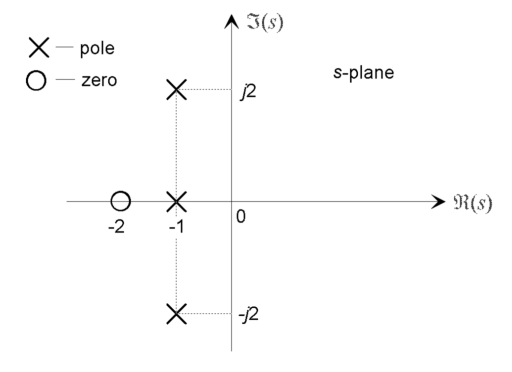
\includegraphics[height=0.5\textheight]{../figs/Ejemplo_PoleZero.pdf}
\end{center}
\end{frame}
\begin{frame}[label={sec:org176ba81}]{La función de transferencia es un fasor}
\begin{itemize}
\item Evaluamos la función de transferencia en el eje imaginario:
\end{itemize}
\[
\laplace{H}\rvert_{\slp = j\omega} = \fasor{H} 
\]
\begin{itemize}
\item Dado que estamos en régimen permanente sinusoidal es \alert{un fasor con módulo y ángulo}:
\end{itemize}
\[
\fasor{H} = H\phase{\phi}
\]

\begin{itemize}
\item Tanto el módulo como el ángulo \alert{varían con la frecuencia}:
\end{itemize}

\[
\fasor{H} \Rightarrow
\begin{cases} 
  |\fasor{H}|\\
  \phi(\omega)
\end{cases}
\]
\end{frame}


\begin{frame}[label={sec:org8457596}]{Interpretación Geométrica}
Cada uno de los factores de \(\laplace{H}\rvert_{\slp = j\omega}\) es un número complejo que conecta un cero/polo con el eje imaginario.
\begin{columns}
\begin{column}[t]{0.3\columnwidth}
\[
\fasor{H} = \frac{j\omega - \mathbf{z_1}}{(j\omega - \mathbf{p_1}) \cdot (j\omega - \mathbf{p_2})}
\]
\end{column}
\begin{column}[t]{0.7\columnwidth}
\begin{center}
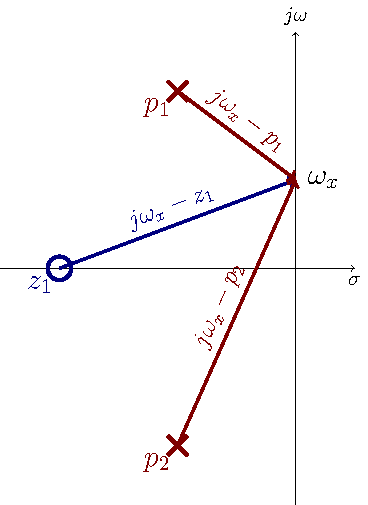
\includegraphics[height=0.8\textheight]{../figs/InterpretacionGeometrica.pdf}
\end{center}
\end{column}
\end{columns}
\end{frame}

\begin{frame}[label={sec:org0127f75}]{Interpretación Geométrica: cero simple}
\[
  \fasor{H} = K \cdot (j\omega - \mathbf{z_1})
\]

\begin{columns}
\begin{column}{0.5\columnwidth}
\begin{center}
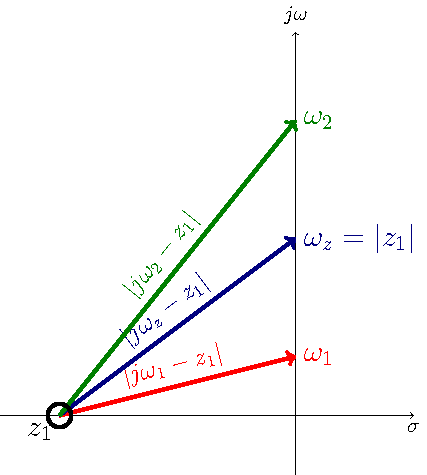
\includegraphics[width=.9\linewidth]{../figs/CeroGeometrica.pdf}
\end{center}
\end{column}

\begin{column}{0.5\columnwidth}
\begin{center}
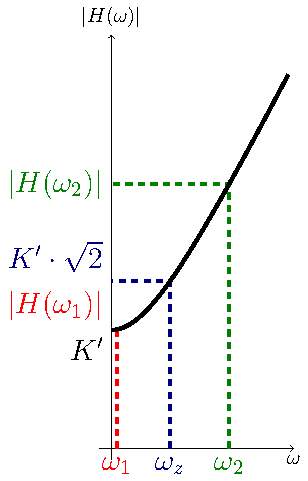
\includegraphics[width=.9\linewidth]{../figs/CeroGeometricaPlot.pdf}
\end{center}
\end{column}
\end{columns}
\end{frame}

\begin{frame}[label={sec:org39257ce}]{Interpretación Geométrica: polo simple}
\[
  \fasor{H} = \frac{K}{j\omega - \mathbf{p_1}}
\]

\begin{columns}
\begin{column}{0.5\columnwidth}
\begin{center}
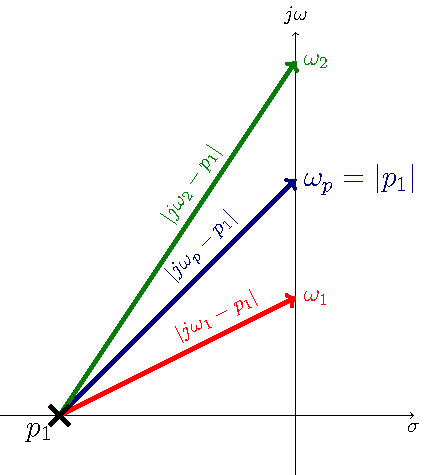
\includegraphics[width=.9\linewidth]{../figs/PoloGeometrica.pdf}
\end{center}
\end{column}

\begin{column}{0.5\columnwidth}
\begin{center}
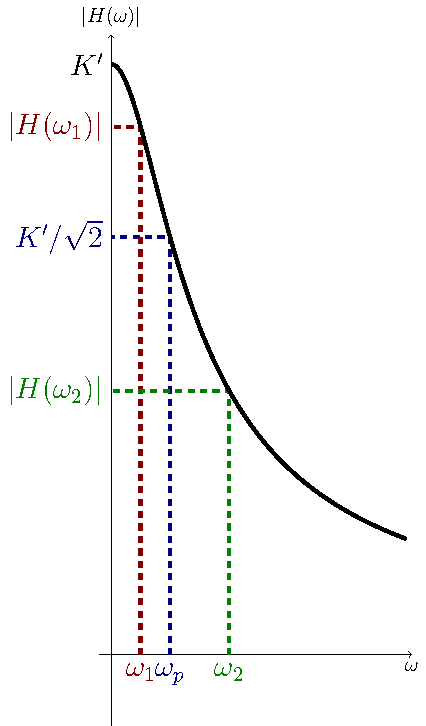
\includegraphics[height=0.6\textheight]{../figs/PoloGeometricaPlot.pdf}
\end{center}
\end{column}
\end{columns}
\end{frame}

\begin{frame}[label={sec:org9f01a96}]{Ejercicios Recomendados}
\begin{itemize}
\item AS: Ejemplo 14.2.
\item Exámenes:
\begin{itemize}
\item Feb 2004 (a), Jun 2013 (a)
\item Sep 2007 (a), Feb 2005 (a), Feb 2010 (a)
\item Nov 2014 (a), Sep 2005 (a), Sep 2006 (a).
\end{itemize}
\end{itemize}
\end{frame}
\section{Diagrama de Bode}
\label{sec:orged5c197}

\begin{frame}[label={sec:org42a511a}]{Introducción}
\begin{itemize}
\item Un diagrama de Bode representa de forma \alert{aproximada} la magnitud y la fase de la función de transferencia.
\item Son \alert{gráficos semilogarítmicos}:
\begin{itemize}
\item Magnitud en \alert{decibelios} frente al logaritmo de la frecuencia/pulsación.
\item Fase en radianes/grados frente al logaritmo de la frecuencia/pulsación.
\end{itemize}
\end{itemize}
\begin{center}
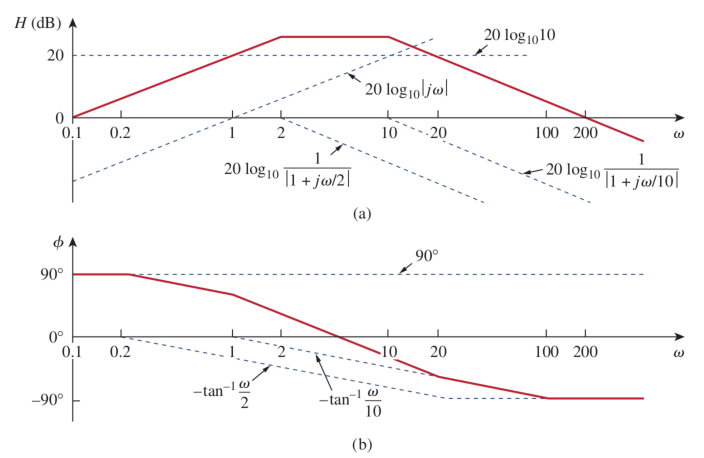
\includegraphics[height=0.5\textheight]{../figs/Bode.pdf}
\end{center}
\end{frame}

\begin{frame}[label={sec:orgb59b4e6}]{Repaso de logaritmos}
\begin{block}{Propiedades}
\begin{align*}
  \log {P_1 \cdot P_2} &= \log P_1 + \log P_2\\
  \log \frac{P_1}{P_2} &= \log P_1 - \log P_2\\
  \log P^n &= n \cdot \log P
\end{align*}
\end{block}

\begin{block}{Valores útiles}
\[
\begin{array}{ll}
  \log 1 = 0 & \log 2 = 0.30103\\
  \log 10 = 1 & \log \frac{1}{2} = -0.30103
\end{array}
\]
\end{block}
\end{frame}

\begin{frame}[label={sec:orged47600}]{Decibelio}
El \alert{decibelio} (\(\si{\decibel}\)) se emplea para medir la ganancia de potencia o la ratio de dos niveles de potencia:

\[
G_{dB} = 10 \log G = 10 \log \frac{P_2}{P_1}
\]

\begin{center}
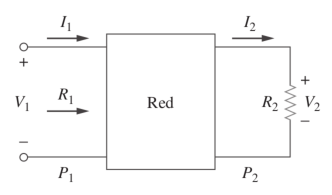
\includegraphics[width=.9\linewidth]{../figs/Red_Ganancia.pdf}
\end{center}
\end{frame}


\begin{frame}[label={sec:org9082dbf}]{Decibelio}
Suponiendo \(R_1 = R_2\), también se emplea para medir la ganancia de tensión/corriente:

\[
G_{dB} = 10 \log \frac{V_2^2}{V_1^2} = 20 \log \frac{V_2}{V_1}
\]

\begin{center}
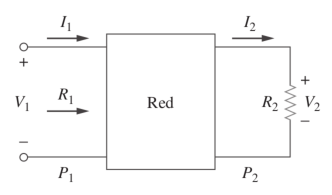
\includegraphics[width=.9\linewidth]{../figs/Red_Ganancia.pdf}
\end{center}
\end{frame}

\begin{frame}[label={sec:orgdb4e13a}]{Valores importantes}
\begin{itemize}
\item Ganancia unidad
\end{itemize}

\[
  G = 1 \Rightarrow
  \left\{
  \begin{array}{c}
    P_1 = P_2\\
    \\
    V_1 = V_2
  \end{array}
  \right\}
  \Rightarrow
  \left\{
  \begin{array}{c}
    G_{dB} = 10 \log \frac{P_2}{P1} = \SI{0}{\decibel}\\
    \\
    G_{dB} = 20 \log \frac{V_2}{V1} = \SI{0}{\decibel}
  \end{array}
  \right\}
\]

\begin{itemize}
\item Potencia Mitad
\end{itemize}

\[
  P_2 = \frac{P_1}{2} \Rightarrow
  \left\{
  \begin{array}{c}
    G = \frac{1}{2}\\
    \\
    V_2 = \frac{V_1}{\sqrt{2}}
  \end{array}
  \right\}
  \Rightarrow
  \left\{
  \begin{array}{c}
    G_{dB} = 10 \log \frac{P_2}{P1} = -\SI{3}{\decibel}\\
    \\
    G_{dB} = 20 \log \frac{V_2}{V_1} = -\SI{3}{\decibel}
  \end{array}
  \right\}
\]
\end{frame}

\begin{frame}[label={sec:org885746c}]{Construcción del Diagrama de Bode}
\begin{itemize}
\item Reescribimos \(\laplace{H}\) de forma normalizada
\end{itemize}
\[
  \laplace{H}\rvert_{\slp =j\omega} = K \frac{(1 + \slp/\omega_{z1}) \cdot (1 + \slp/\omega_{z2}) \ldots (1 + \slp/\omega_{zm})}{(1 + \slp/\omega_{p1}) \cdot (1 + \slp/\omega_{p2}) \ldots (1 + \slp/\omega_{pn})} 
\]
\begin{itemize}
\item Módulo
\end{itemize}
\[
  |\fasor{H}| = K \frac{|1 + j\omega/\omega_{z1}| \cdot |1 + j\omega/\omega_{z2}| \ldots |1 + j\omega/\omega_{zm}|}{|1 + j\omega/\omega_{p1}| \cdot |1 + j\omega/\omega_{p2}| \ldots |1 + j\omega/\omega_{pn}|} 
\]

\begin{itemize}
\item Ángulo
\end{itemize}
\begin{align*}
\phi(\omega) &= \atan(\omega/\omega_{z1}) + \atan(\omega/\omega_{z2}) + \ldots + \atan(\omega/\omega_{zm}) - \\
&- \left(\atan(\omega/\omega_{p1}) + \atan(\omega/\omega_{p2}) + \ldots + \atan(\omega/\omega_{pn})\right) 
\end{align*}
\end{frame}

\begin{frame}[label={sec:org8c969b0}]{Construcción del Diagrama de Bode}
\begin{itemize}
\item Al aplicar logaritmos a la expresión de la amplitud \alert{los productos se convierten en sumas}.
\item La estrategia de construcción consiste en analizar la \alert{contribución de cada cero/polo por separado} y \alert{sumar} para obtener el resultado global.
\end{itemize}

\begin{center}
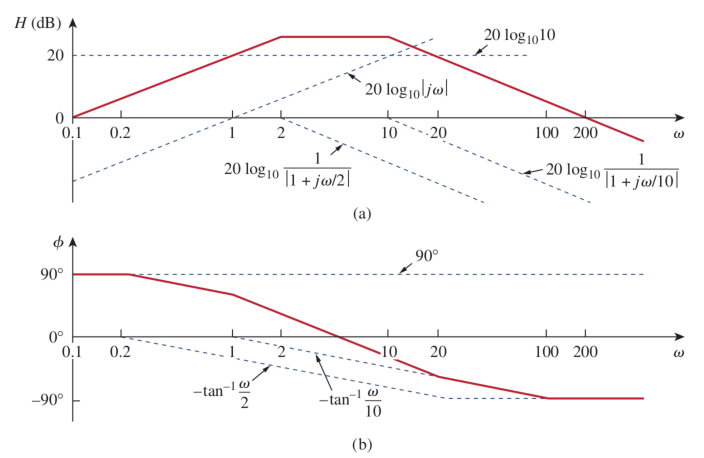
\includegraphics[height=0.5\textheight]{../figs/Bode.pdf}
\end{center}
\end{frame}

\begin{frame}[label={sec:org2ae0115}]{Construcción del Diagrama de Bode}
\begin{block}{Posibilidades}
\begin{itemize}
\item Término constante: \(K\)
\item Cero/Polo en el origen: \(j\omega\)
\item Cero/Polo simple: \(1 + j\omega/\omega_c\)
\item Cero/Polo múltiple (\emph{raíces reales repetidas}): \((1 + j\omega/\omega_c)^N\)
\item Cero/Polo cuadrático (\emph{raíces complejas conjugadas}): \(1 - (\omega/\omega_0)^2 + j2\zeta\omega/\omega_0\)
\end{itemize}
\end{block}
\end{frame}

\begin{frame}[label={sec:org9fb9238}]{Término Constante}
\[
  \fasor{H} = K \Rightarrow
  \begin{cases}
    |\fasor{H}| = 20 \log |K|\\
    \phi(\omega) = 
    \begin{cases}
      \ang{0} \quad si \quad K > 0\\
      \ang{180} \quad si \quad K < 0\\
    \end{cases}
  \end{cases}
\]

\begin{center}
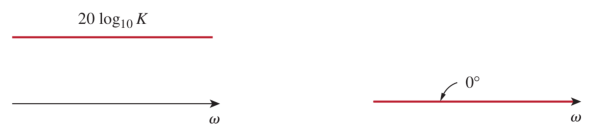
\includegraphics[width=.9\linewidth]{../figs/BodeConstante.pdf}
\end{center}
\end{frame}

\begin{frame}[label={sec:orgaf868c1}]{Cero en el origen\footnote{\alert{Atención}: el origen \(\omega = 0\) no se representa en una escala logarítmica.}}
\[
  \fasor{H} = j\omega \Rightarrow
  \begin{cases}
    |\fasor{H}| = 20 \log \omega\\
    \phi(\omega) = \ang{90}
  \end{cases}
\]



\begin{center}
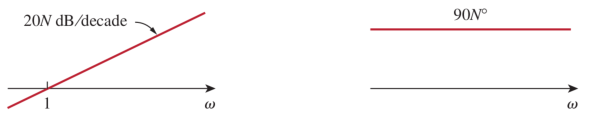
\includegraphics[width=.9\linewidth]{../figs/BodeCeroOrigen.pdf}
\end{center}

Década: rango de frecuencias comprendido entre \(\omega_1\) y \(10\cdot\omega_1\).
\end{frame}

\begin{frame}[label={sec:org13f097d}]{Polo en el origen}
\[
  \fasor{H} = \frac{1}{j\omega} \Rightarrow
  \begin{cases}
    |\fasor{H}| = - 20 \log \omega\\
    \phi(\omega) = - \ang{90}
  \end{cases}
\]

\begin{center}
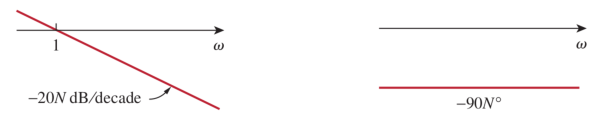
\includegraphics[width=.9\linewidth]{../figs/BodePoloOrigen.pdf}
\end{center}
\end{frame}

\begin{frame}[label={sec:orge8f6003}]{Cero simple}
\[
  \fasor{H} = 1 + j\frac{\omega}{\omega_z} \Rightarrow
  \begin{cases}
    |\fasor{H}| =  20 \log \sqrt{1 + \left(\frac{\omega}{\omega_z}\right)^2}\\
    \phi(\omega) = \atan(\frac{\omega}{\omega_z}) 
  \end{cases}
\]

\[
  |\fasor{H}| = 
  \begin{cases}
  20 \log 1 = 0, \quad \omega \to 0\\
  20 \log \frac{\omega}{\omega_z}, \quad \omega \gg \omega_z\\
  \end{cases}
\]

\[
  \phi(\omega) = 
  \begin{cases}
    \ang{0},\quad \omega \leq 0.1\omega_z\\
    \ang{45}, \quad \omega = \omega_z\\
    \ang{90}, \quad \omega \geq 10\omega_z\\
  \end{cases}
\]

\begin{center}
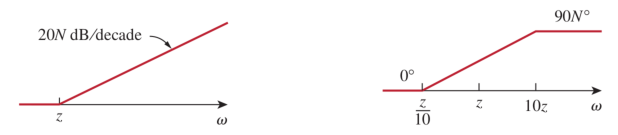
\includegraphics[width=.9\linewidth]{../figs/BodeCeroSimple.pdf}
\end{center}
\end{frame}

\begin{frame}[label={sec:orgd8a55ea}]{Polo simple}
\[
  \fasor{H} = \frac{1}{1 + j\frac{\omega}{\omega_p}} \Rightarrow
  \begin{cases}
    |\fasor{H}| =  - 20 \log \sqrt{1 + \left(\frac{\omega}{\omega_p}\right)^2}\\
    \phi(\omega) = - \atan(\frac{\omega}{\omega_p}) 
  \end{cases}
\]

\[
  |\fasor{H}| = 
  \begin{cases}
  - 20 \log 1 = 0, \quad \omega \to 0\\
  - 20 \log \frac{\omega}{\omega_p}, \quad \omega \gg \omega_p\\
  \end{cases}
\]

\[
  \phi(\omega) = 
  \begin{cases}
    \ang{0},\quad \omega \leq 0.1\omega_p\\
    - \ang{45}, \quad \omega = \omega_p\\
    - \ang{90}, \quad \omega \geq 10 \omega_p
  \end{cases}
\]


\begin{center}
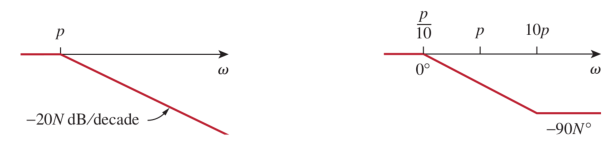
\includegraphics[width=.9\linewidth]{../figs/BodePoloSimple.pdf}
\end{center}
\end{frame}

\begin{frame}[label={sec:org2210e88}]{Cero cuadrático}
Sea \(\laplace{H}\rvert_{\slp = j\omega}  = \slp^2 + 2\alpha \slp + \omega_0^2\), con \(\alpha < \omega_0\). Usando \(\zeta = \alpha/\omega_0 < 1\) y normalizando:

\[
  \fasor{H} = 1 + j 2 \zeta \frac{\omega}{\omega_0} - \left(\frac{\omega}{\omega_0}\right)^2 
\]


\[
  |\fasor{H}| = 
  \begin{cases}
  20 \log 1 = 0, \quad \omega \to 0\\
  40 \log (\omega/\omega_0), \quad \omega \gg \omega_0\\
  \end{cases}
\]

\[
  \phi(\omega) = \atan \frac{2\zeta\omega/\omega_0}{1 - \omega^2/\omega_0^2}
  \begin{cases}
    \ang{0},\quad \omega \leq 0.1\omega_0\\
    \ang{90}, \quad \omega = \omega_0\\
    \ang{180}, \quad \omega \geq 10 \omega_0
  \end{cases}
\]


\begin{center}
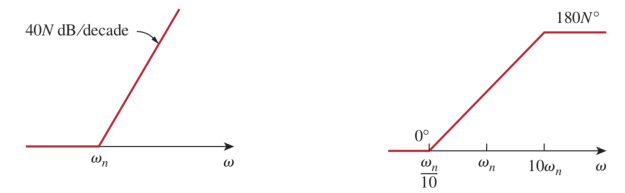
\includegraphics[width=.9\linewidth]{../figs/BodeCeroCuadratico.pdf}
\end{center}
\end{frame}


\begin{frame}[label={sec:org0720aa2}]{Polo cuadrático}
\[
  \fasor{H} = \frac{1}{1 + j 2 \zeta \frac{\omega}{\omega_0} - \left(\frac{\omega}{\omega_0}\right)^2} 
\]


\[
  |\fasor{H}| = 
  \begin{cases}
  - 20 \log 1 = 0, \quad \omega \to 0\\
  - 40 \log (\omega/\omega_0), \quad \omega \gg \omega_0\\
  \end{cases}
\]

\[
  \phi(\omega) = - \atan \frac{2\zeta\omega/\omega_0}{1 - \omega^2/\omega_0^2}
  \begin{cases}
    \ang{0},\quad \omega \leq 0.1\omega_0\\
    - \ang{90}, \quad \omega = \omega_0\\
    - \ang{180}, \quad \omega \geq 10 \omega_0
  \end{cases}
\]



\begin{center}
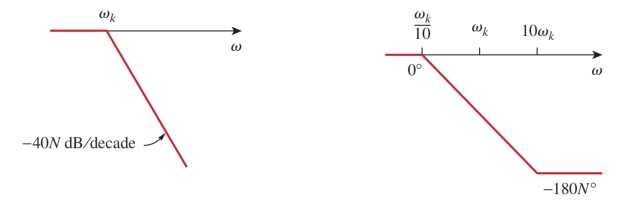
\includegraphics[width=.9\linewidth]{../figs/BodePoloCuadratico.pdf}
\end{center}
\end{frame}

\begin{frame}[label={sec:orgb29760a}]{Ejercicios Recomendados}
\begin{itemize}
\item AS: ejemplos 14.3, 14.4, 14.5, 14.6.
\item Exámenes:
\begin{itemize}
\item Feb 2004 (b), Jun 2013 (b)
\item Sep 2007 (b), Feb 2005 (b), Feb 2010 (b)
\item Nov 2014 (b), Sep 2005 (b), Sep 2006 (b).
\end{itemize}
\end{itemize}
\end{frame}
\section{Filtros}
\label{sec:org5b55206}
\begin{frame}[label={sec:orge4ca6bc}]{Filtro Paso Bajo}
\begin{columns}
\begin{column}{0.3\columnwidth}
\begin{align*}
  |H(0)| &= 1\\
  |H(\omega_c)| &= 1/\sqrt{2}\\
  |H(\infty)| &= 0
\end{align*}
\end{column}
\begin{column}{0.7\columnwidth}
\begin{center}
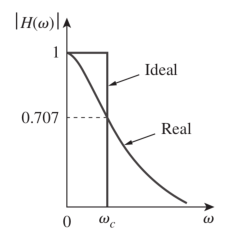
\includegraphics[width=.9\linewidth]{../figs/Filtro_PasoBajo.pdf}
\end{center}
\end{column}
\end{columns}
\end{frame}

\begin{frame}[label={sec:orgfbd278c}]{Filtro Paso Alto}
\begin{columns}
\begin{column}{0.3\columnwidth}
\begin{align*}
  |H(0)| &= 0\\
  |H(\omega_c)| &= 1/\sqrt{2}\\
  |H(\infty)| &= 1
\end{align*}
\end{column}

\begin{column}{0.7\columnwidth}
\begin{center}
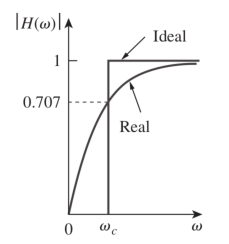
\includegraphics[width=.9\linewidth]{../figs/Filtro_PasoAlto.pdf}
\end{center}
\end{column}
\end{columns}
\end{frame}

\begin{frame}[label={sec:orgf1ceb69}]{Filtro Paso Banda}
\begin{columns}
\begin{column}{0.3\columnwidth}
\begin{align*}
  |H(\omega < \omega_1)| &= 0\\
  |H(\omega_1 < \omega < \omega_2)| &= 1\\
  |H(\omega > \omega_2)| &= 0
\end{align*}
\end{column}

\begin{column}{0.7\columnwidth}
\begin{center}
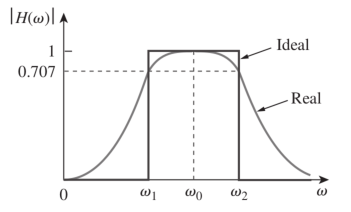
\includegraphics[width=.9\linewidth]{../figs/Filtro_PasoBanda.pdf}
\end{center}
\end{column}
\end{columns}
\end{frame}

\begin{frame}[label={sec:org0bf1354}]{Filtro Banda Eliminada}
\begin{columns}
\begin{column}{0.3\columnwidth}
\begin{align*}
  |H(\omega < \omega_1)| &= 1\\
  |H(\omega_1 < \omega < \omega_2)| &= 0\\
  |H(\omega > \omega_2)| &= 1
\end{align*}
\end{column}

\begin{column}{0.7\columnwidth}
\begin{center}
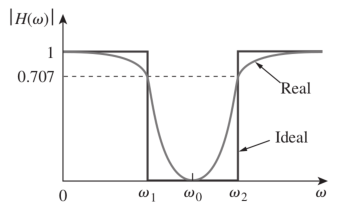
\includegraphics[width=.9\linewidth]{../figs/Filtro_BandaEliminada.pdf}
\end{center}
\end{column}
\end{columns}
\end{frame}

\begin{frame}[label={sec:org232652a}]{Ejemplo: circuito RC}
\begin{columns}
\begin{column}{0.5\columnwidth}
\begin{center}
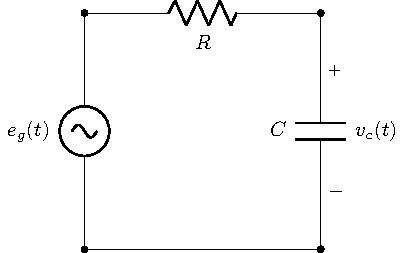
\includegraphics[width=.9\linewidth]{../figs/filtroRC.pdf}
\end{center}
\end{column}

\begin{column}{0.5\columnwidth}
\begin{center}
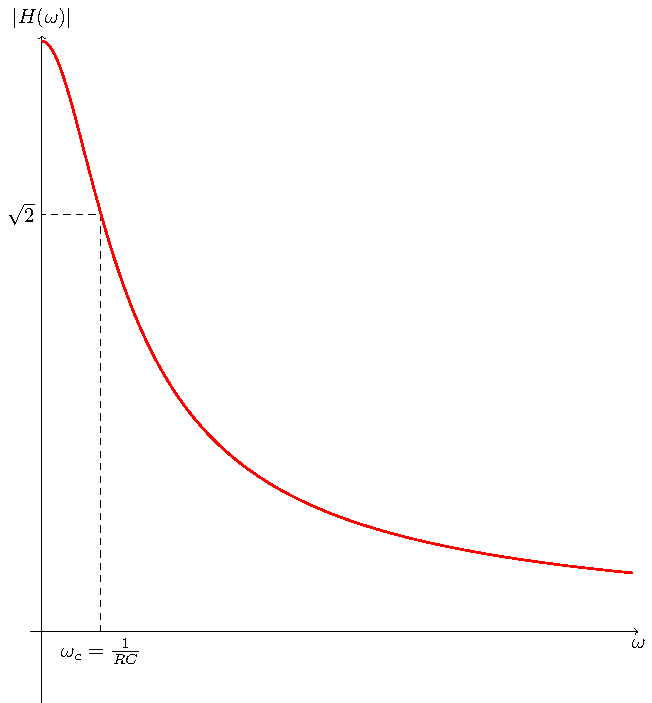
\includegraphics[width=.9\linewidth]{../figs/Hw_RC.pdf}
\end{center}
\end{column}
\end{columns}

\[
\laplace{H} = \frac{\laplace{U_c}}{\laplace{E_g}} \Rightarrow |\fasor{H}| = \frac{1}{\sqrt{1 + (\omega/\omega_c)^2}} 
\]
\end{frame}

\begin{frame}[label={sec:orgb27603b}]{Ejemplo: circuito RL}
\begin{columns}
\begin{column}{0.5\columnwidth}
\begin{center}
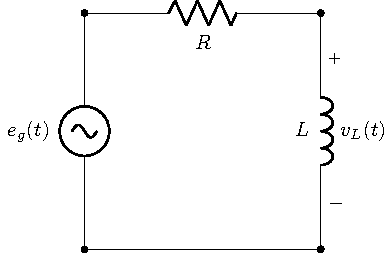
\includegraphics[width=.9\linewidth]{../figs/filtroRL.pdf}
\end{center}
\end{column}

\begin{column}{0.5\columnwidth}
\begin{center}
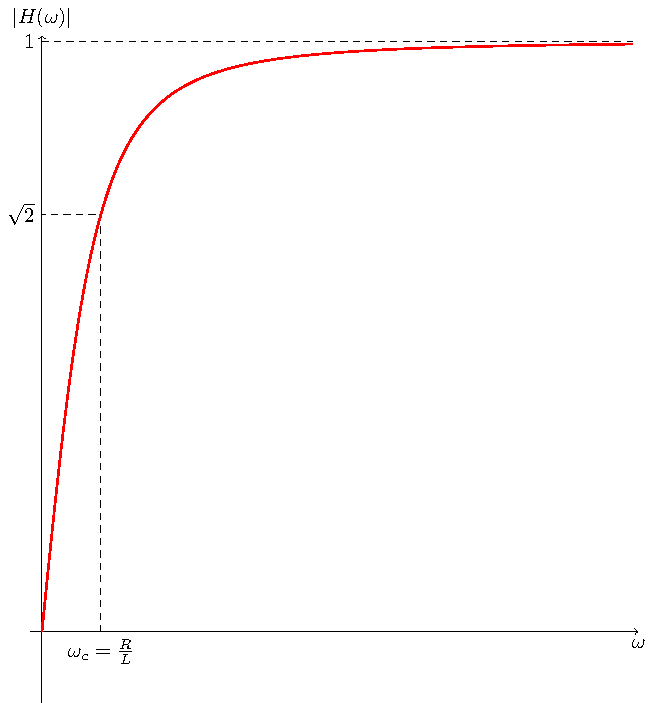
\includegraphics[width=.9\linewidth]{../figs/Hw_RL.pdf}
\end{center}
\end{column}
\end{columns}

\[
\laplace{H} = \frac{\laplace{U_L}}{\laplace{E_g}} \Rightarrow |\fasor{H}| = \frac{\omega/\omega_c}{\sqrt{1 + (\omega/\omega_c)^2}} 
\]
\end{frame}

\begin{frame}[label={sec:org0d3e256}]{Circuitos para practicar}
\begin{columns}
\begin{column}{0.5\columnwidth}
\[
  \fasor{H} = \frac{\fasor{U_R}}{\fasor{E_g}}
\]
\begin{center}
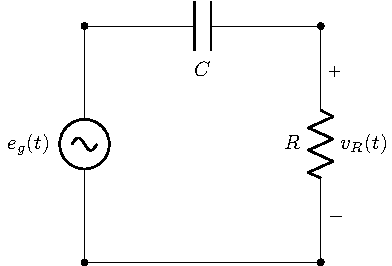
\includegraphics[width=.9\linewidth]{../figs/filtroCR.pdf}
\end{center}
\end{column}
\begin{column}{0.5\columnwidth}
\[
  \fasor{H} = \frac{\fasor{U_R}}{\fasor{E_g}}
\]
\begin{center}
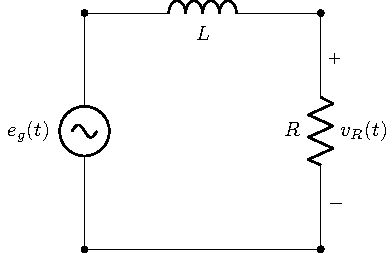
\includegraphics[width=.9\linewidth]{../figs/filtroLR.pdf}
\end{center}
\end{column}
\end{columns}
\end{frame}
\end{document}